% PyGeoParallax-IN manuscript, prepared for Atmospheric Measurement Techniques (AMT, Copernicus).
% Back matter follows AMT's required sections. For submission, move the text into the Copernicus
% LaTeX template (copernicus.cls) from https://publications.copernicus.org/for_authors/manuscript_preparation.html
% Compile with pdfLaTeX + BibTeX (Overleaf default). Sections 2-6 are generated from the
% Markdown drafts by 08_manuscript/md_to_latex.py; edit those drafts or the .tex files here.
\documentclass[11pt,a4paper]{article}

\usepackage[utf8]{inputenc}
\usepackage[T1]{fontenc}
\usepackage{lmodern}
\usepackage{textcomp}
\usepackage{amsmath,amssymb}
\usepackage{graphicx}
\usepackage{booktabs,longtable,array,calc}
\usepackage[margin=2.5cm]{geometry}
\usepackage[authoryear,round]{natbib}
\usepackage{xcolor}
\usepackage[colorlinks=true,linkcolor=blue!50!black,citecolor=blue!50!black,urlcolor=blue!50!black]{hyperref}
\usepackage{newunicodechar}

% Characters used in the generated sections.
\newunicodechar{°}{\textdegree}
\newunicodechar{−}{\ensuremath{-}}
\newunicodechar{±}{\ensuremath{\pm}}
\newunicodechar{µ}{\textmu}
\newunicodechar{≥}{\ensuremath{\geq}}
\newunicodechar{·}{\ensuremath{\cdot}}
\newunicodechar{→}{\ensuremath{\rightarrow}}
\newunicodechar{ρ}{\ensuremath{\rho}}

% Pandoc output helpers.
\providecommand{\tightlist}{\setlength{\itemsep}{0pt}\setlength{\parskip}{0pt}}
\newcommand{\passthrough}[1]{#1}
\providecommand{\doi}[1]{\href{https://doi.org/#1}{doi:#1}}
\setlength{\LTcapwidth}{\textwidth}

\title{Parallax correction of INSAT-3DR imagery over India:\\an open-source tool and the limits of validation against GPM radar}
\author{Naveen Bapalli\thanks{Independent researcher, India. Correspondence: Naveen Bapalli ([e-mail to be added]).}}
\date{Manuscript for \textit{Atmospheric Measurement Techniques}, \today}

\begin{document}
\maketitle

\begin{abstract}
Geostationary imagers see high clouds displaced away from the sub-satellite point. For INSAT-3DR at 74\,\textdegree E, deep convection over the Himalaya and Northeast India appears about 10\,km from its true position, two to three infrared pixels. We present PyGeoParallax-IN, an open-source Python tool that corrects this parallax for INSAT-3DR imagery. It estimates cloud-top height from 10.8\,\textmu m brightness temperature, traces each line of sight to the cloud top on the WGS84 ellipsoid (with terrain if a digital elevation model is given), applies a navigation correction measured from coastlines, and regrids the scene so that uncorrected and corrected datasets share one grid.

We validate the correction against GPM Ku-band radar in 33 coincident monsoon cases (2022--2024) over South, Central and Northeast India and the Himalaya, 14 of them usable. Parallax correction lowers the median INSAT--GPM storm-top offset from 5.5 to 3.1\,km (10 of 12 cases improve; sign test $p=0.039$) and leaves the cross-look offset unchanged. At storm cores, however, a parallax-only correction overshoots by about 5.7\,km: INSAT-3DR L1C positions carry a seasonal navigation error, 7--20\,km to the west in winter and 2.5--5\,km to the south in the monsoon, which partly cancels the parallax. Correcting navigation as well reduces the overshoot significantly and gives a median field offset of 1.8\,km, although with 12 cases this is not significantly better than parallax correction alone. ERA5 profiles and SRTM terrain change the storm results by less than 0.5\,km. The tool processes an India scene in 1.8\,s.
\end{abstract}


\noindent\textbf{Keywords:} parallax correction; INSAT-3DR; geostationary satellite; navigation error; GPM DPR; Indian monsoon; open-source software

\section{Introduction}
\label{sec:introduction}

Geostationary satellites observe the Indian monsoon every 15--30 minutes and are the only source of continuous cloud and rainfall information over much of South Asia. Their images are geolocated as if every pixel lay on the Earth's surface. A cloud top several kilometres high lies on the same line of sight but closer to the satellite, so it appears displaced away from the sub-satellite point by about $h\tan(\mathrm{VZA})$, where $h$ is the cloud-top height and VZA the viewing zenith angle. This parallax displacement is zero below the satellite and grows towards the edge of the disk.

India is unusually exposed to this effect. INSAT-3DR, the operational Indian geostationary imager, sits at 74\,\textdegree E, close to the western edge of the country. Its viewing angle reaches 33--38\textdegree{} over the Himalaya and Northeast India, where monsoon convection reaches the tropopause at 15--17\,km. Deep convective tops there appear 8--12\,km from their true position, two to three infrared pixels. Products that use INSAT-3DR imagery, from rainfall estimates to cloud masks and machine-learning classifications of precipitation type, inherit this displacement, and comparisons with radar or rain gauges mix it with any real error.

Parallax correction is well established elsewhere. \citet{vicente2002} showed its importance for satellite rainfall estimates, and their correction has been used operationally in the GOES Hydro-Estimator since 2001 \citep{scofield2003}. \citet{bielinski2020} derived an accurate geometric solution on the ellipsoid and validated it against ground radar over Europe. An open-source correction exists in satpy \citep{raspaud2018,satpy_parallax}, which assumes a spherical Earth and does not handle terrain. For INSAT-3D and INSAT-3DR, however, we found no published parallax correction or validation.

Validating a parallax correction is harder than it seems. A radar measures precipitation, not cloud top, and geolocation errors of the imager mix with the parallax. ISRO's data-quality reports measure INSAT-3DR geolocation error against ground control points; for full-disk images in June 2020 it was 1.7--2.7 infrared pixels to the north \citep{mosdac_dqe2020}, comparable to the parallax itself. How the INSAT--radar offset responds to a parallax correction, and how much of the correction a radar can verify, has not been examined for India.

This paper addresses both the correction and its verification. Our contributions are:
\begin{enumerate}
  \item \textbf{An open-source tool, PyGeoParallax-IN} \citep{pygeoparallax}. It corrects INSAT-3DR imagery for parallax by exact ray tracing on the WGS84 ellipsoid, optionally with terrain, and applies a navigation correction measured from coastlines. It produces uncorrected and corrected datasets on the same grid with occlusion-aware resampling.
  \item \textbf{A validation against GPM Ku-band radar} in 63 coincident monsoon cases (2018--2024; 38 usable) across four Indian regions that span the full range of viewing angles. It uses two independent offset measures, at the scale of the storm and of the convective core.
  \item \textbf{A test of what radar validation can resolve.} Most of the computed parallax is not visible against GPM at convective cores. With a synthetic test and a navigation correction fitted to GPM, we show that this is not a method error and cannot be explained by navigation alone, and that storm structure limits GPM-based validation of absolute position to about $\pm$3--5\,km.
  \item \textbf{A characterisation of INSAT-3DR L1C navigation error} and of the remaining error sources: cloud-top height (standard atmosphere versus ERA5), terrain (SRTM) and the slanted GPM radar beam.
\end{enumerate}

Section~\ref{sec:data} describes the data, Section~\ref{sec:method} the correction method and Section~\ref{sec:validation} the validation design. Section~\ref{sec:results} presents the results, Section~\ref{sec:discussion} discusses them, and Section~\ref{sec:conclusions} concludes.

\section{Data}
\label{sec:data}
\label{sec:2}

\subsection{INSAT-3DR Imager}\label{sec:2.1}

INSAT-3DR is a geostationary satellite at 74.0°E. Its Imager scans the full disk every 30 minutes (scans start at HH:15 and HH:45) in six channels: visible (VIS, 0.65 µm), shortwave infrared (SWIR, 1.6 µm), mid-wave infrared (MIR, 3.9 µm), water vapour (WV, 6.8 µm) and two thermal infrared channels (TIR1, 10.8 µm; TIR2, 12.0 µm). The sampling interval is 1 km for VIS and SWIR and 4 km for the infrared channels at the sub-satellite point. We used the Level-1C sector product (\texttt{3RIMG\_*\_L1C\_SGP}) from MOSDAC; INSAT-3DR products use the INSAT-3D formats \citep{sac2014}. It is on a Mercator grid (\texttt{lon\_0\ =\ 75°E}) with pixel-centre coordinates. Calibrated counts are converted to brightness temperature (BT) or albedo through the lookup tables in each file.

The full-disk scan runs north to south, from 81°N to 81°S, in about 26.9 min (from the file start and end times). We estimate the scan time at a given latitude by linear interpolation along this sweep.

We did not use the satellite elevation and azimuth angles in the L1C files: they differ from the geometric values by about 1°. Viewing angles are computed directly (Section~\ref{sec:3.1}).

The Level-2B cloud-top pressure product (\texttt{3RIMG\_*\_L2B\_CTP}) gives cloud-top pressure and temperature in coarse boxes (about 37 km) and a clear-sky brightness temperature (CSBT) per channel. It contains no cloud-top height. We use its CSBT as the clear-sky reference for the cloud mask (Section~\ref{sec:3.2}) and its cloud-top pressure only as a cross-check. Its sub-satellite longitude attribute (82°E) is incorrect for INSAT-3DR and is ignored.

\subsection{GPM Dual-frequency Precipitation Radar}\label{sec:2.2}

GPM Core Observatory carries the Dual-frequency Precipitation Radar (DPR) \citep{hou2014}. We used the Ku-band Level-2A product (\texttt{2A.GPM.Ku}, version V08 \citep{gpm2aku_v08}; algorithm in \citet{iguchi2021}) from NASA GES DISC, full-swath (\texttt{FS}) group, about 245 km wide with a footprint of about 5 km. Variables read: storm-top height, near-surface corrected reflectivity, near-surface precipitation rate, precipitation type, bright-band height and the spacecraft position.

GPM 2A gives each footprint's position at the surface. An echo at height \(h\) lies on the slanted radar beam, displaced towards the spacecraft by about \(h\tan\theta_{\mathrm{GPM}}\), where \(\theta_{\mathrm{GPM}}\) is the local zenith angle of the beam. This displacement is up to about 5 km for a 15 km storm top at the swath edge. We place storm tops on the beam by intersecting the line from the footprint to the spacecraft with the ellipsoid surface at height \(h\), using the same Newton refinement as in Section~\ref{sec:3.3}. The median displacement in our cases is 1 km.

\subsection{Ancillary data}\label{sec:2.3}

\begin{itemize}
\tightlist
\item
  \textbf{Coastlines:} Natural Earth 10 m land polygons (public domain) \citep{naturalearth}, used for the navigation check (Section~\ref{sec:3.6}).
\item
  \textbf{Atmospheric profiles:} AFGL tropical standard atmosphere \citep{anderson1986}, 0--25 km at 1 km resolution; and ERA5 reanalysis \citep{hersbach2020,c3s2018} temperature and geopotential on 29 pressure levels (1000--50 hPa, 0.25°), at the hour nearest each case scan.
\item
  \textbf{Terrain:} SRTM GL1 \citep{farr2007}, 1 arcsecond tiles block-averaged to 0.01° (about 1 km). Heights are above the EGM96 geoid, which lies 50--105 m below the ellipsoid over India; this changes the terrain correction by under 75 m at VZA 35°, so heights are used as they are.
\end{itemize}

\subsection{Study period and regions}\label{sec:2.4}

The study covers the monsoon season (June--September) of 2022, 2023 and 2024. Validation cases come from four regions that span the range of INSAT-3DR viewing angles over India:

\begin{longtable}[]{@{}
  >{\raggedright\arraybackslash}p{(\linewidth - 4\tabcolsep) * \real{0.3333}}
  >{\raggedright\arraybackslash}p{(\linewidth - 4\tabcolsep) * \real{0.3333}}
  >{\raggedright\arraybackslash}p{(\linewidth - 4\tabcolsep) * \real{0.3333}}@{}}
\caption{Validation regions.}\label{tab:R}\\
\toprule\noalign{}
\begin{minipage}[b]{\linewidth}\raggedright
Region
\end{minipage} & \begin{minipage}[b]{\linewidth}\raggedright
Box (lat, lon)
\end{minipage} & \begin{minipage}[b]{\linewidth}\raggedright
Viewing zenith angle
\end{minipage} \\
\midrule\noalign{}
\endhead
\bottomrule\noalign{}
\endlastfoot
South India (Kerala, Karnataka, Tamil Nadu) & 8--17°N, 74--80.5°E & 9--20° \\
Central India (Madhya Pradesh, Chhattisgarh) & 19--26°N, 76--85°E & 21--30° \\
Himalaya (Uttarakhand, Himachal, Nepal) & 27--33°N, 75--89°E & 31--38° \\
Northeast India and Bangladesh & 22--29°N, 89--97°E & 33--37° \\
\end{longtable}


% Schematic of cloud and terrain parallax (scripts/make_paper_figures.py, fig0_schematic).
\begin{figure}[tbp]
  \centering
  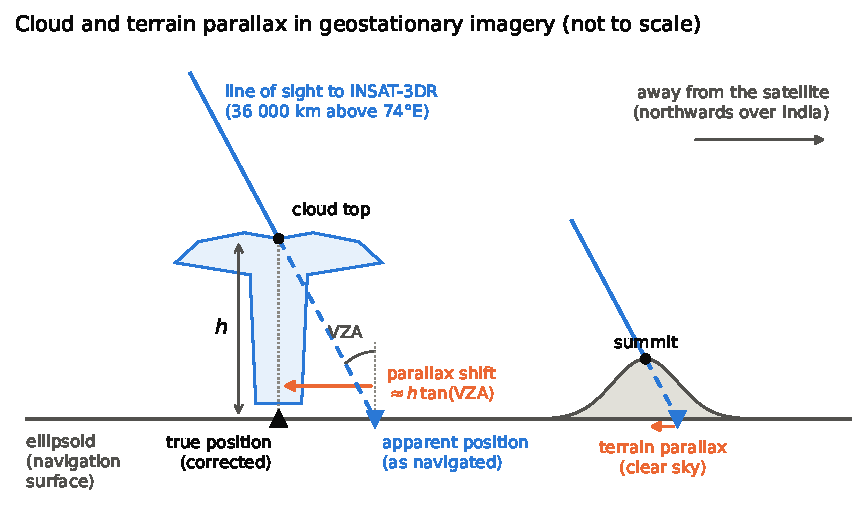
\includegraphics[width=\textwidth]{figures/fig0_schematic.pdf}
  \caption{Cloud and terrain parallax in geostationary imagery (cross-section, not to scale). A cloud top at height $h$ is seen along the line of sight from the satellite and is navigated to where that line meets the ellipsoid (apparent position), displaced away from the satellite by about $h\tan(\mathrm{VZA})$. The correction moves it back to the point on the line of sight at height $h$ (true position). Elevated terrain is displaced in the same way in clear sky.}
  \label{fig:schematic}
\end{figure}

\section{Parallax correction method}
\label{sec:method}
\label{sec:3}

\subsection{Viewing geometry}\label{sec:3.1}

All positions are geodetic coordinates on the WGS84 ellipsoid \citep{nima2000}. A surface point at latitude \(\varphi\), longitude \(\lambda\) and ellipsoidal height \(h\) has Earth-centred, Earth-fixed (ECEF) coordinates

\[
\mathbf{p} = \begin{pmatrix} (N + h)\cos\varphi\cos\lambda \\ (N + h)\cos\varphi\sin\lambda \\ \left(N(1 - e^2) + h\right)\sin\varphi \end{pmatrix},
\qquad N = \frac{a}{\sqrt{1 - e^2\sin^2\varphi}},
\]

with semi-major axis \(a\) and eccentricity \(e\). The inverse transform uses three fixed-point iterations on latitude. Both directions agree with pyproj \citep{pyproj} to better than 1 mm.

The satellite is at \(\mathbf{s} = R_{\mathrm{geo}}(\cos\lambda_s, \sin\lambda_s, 0)\), with \(R_{\mathrm{geo}} = 42\,164\) km and \(\lambda_s = 74.0^\circ\). The unit line-of-sight vector from the ground to the satellite is \(\hat{\mathbf{d}} = (\mathbf{s} - \mathbf{p})/\lVert\mathbf{s} - \mathbf{p}\rVert\). The viewing zenith angle (VZA) is the angle between \(\hat{\mathbf{d}}\) and the local vertical; the viewing azimuth angle (VAA) comes from its east and north components. These agree with pyorbital \citep{raspaud2018} within 0.01°.

A cloud at height \(h\) appears displaced away from the satellite by approximately

\[
\Delta \approx h \tan(\mathrm{VZA}).
\]

Uncorrected, this displacement misplaces satellite rainfall estimates by several kilometres, especially for deep convection at high viewing angles \citep{vicente2002}. Over India the displacement is mostly northward. For a 12 km cloud top it is about 2.6 km at Kochi (VZA 12°) and 8--9 km over Northeast India and the Himalaya (VZA 34--36°).

\subsection{Cloud-top height}\label{sec:3.2}

Cloud-top height is estimated per pixel from TIR1 brightness temperature. For an opaque cloud, TIR1 BT is close to the cloud-top temperature, so the cloud-top height is the height at which the reference profile has that temperature.

\begin{enumerate}
\def\labelenumi{\arabic{enumi}.}
\tightlist
\item
  \textbf{Cloud mask.} A pixel is cloudy if its BT is more than 8 K below the ISRO clear-sky BT, sampled to the pixel by nearest neighbour. Where no clear-sky BT is available, a pixel is cloudy if BT \textless{} 270 K. Clear pixels get no height and are not moved.
\item
  \textbf{Height lookup.} BT is interpolated linearly in the AFGL tropical profile between the surface and the cold-point tropopause (17 km, 194.8 K). BT colder than the tropopause minimum, as in overshooting tops, is assigned the tropopause height.
\end{enumerate}

As an alternative, ERA5 profiles are interpolated bilinearly to each pixel, with geopotential converted to geometric height. The lookup then runs downwards from each column's cold-point tropopause (searched up to 70 hPa), so low-level inversions cannot capture high clouds. On the 14 validation cases, ERA5 changes cold-core heights by −0.15 km (median) and the INSAT--GPM offsets by under 0.5 km relative to the standard atmosphere.

Profile heights are above mean sea level. We treat them as ellipsoidal heights. The difference (the geoid undulation, −50 to −100 m over India) changes the shift by less than 1\%.

The approach has known limits: semi-transparent cirrus appears warmer than its true top, so its height is underestimated; and the standard atmosphere differs from the real one by a few hundred metres.

\subsection{Ray-tracing solver}\label{sec:3.3}

The navigated (apparent) position of a pixel is where its line of sight meets the ellipsoid. A cloud at height \(h\) lies on the same line of sight, nearer the satellite. The corrected position is therefore the point

\[
\mathbf{q}(t) = \mathbf{p}_0 + t\,\hat{\mathbf{d}}
\]

on the line of sight whose geodetic height equals \(h\). Here \(\mathbf{p}_0\) is the apparent position at the navigation reference height \(h_0\) (\(h_0 = 0\) for L1C data).

We follow \citet{bielinski2020} in two steps:

\begin{enumerate}
\def\labelenumi{\arabic{enumi}.}
\tightlist
\item
  \textbf{Enlarged ellipsoid.} Intersect the line with the ellipsoid of semi-axes \(a + h\) and \(b + h\): \[
  \frac{q_x^2 + q_y^2}{(a + h)^2} + \frac{q_z^2}{(b + h)^2} = 1.
  \] This is a quadratic in \(t\), \(A t^2 + B t + C = 0\). We take the root closest to the apparent point, using the numerically stable form \(t = C/q\) or \(q/A\) with \(q = -\tfrac{1}{2}\left(B + \operatorname{sign}(B)\sqrt{B^2 - 4AC}\right)\). The enlarged ellipsoid is not a surface of constant geodetic height, but the error is only about 1 cm for a 12 km cloud over India.
\item
  \textbf{Newton refinement.} One step on the true geodetic height, \[
  t \leftarrow t + \frac{h - h_{\mathrm{geod}}(\mathbf{q}(t))}{\hat{\mathbf{d}}\cdot\hat{\mathbf{u}}(\mathbf{q}(t))},
  \] where \(\hat{\mathbf{u}}\) is the local vertical at \(\mathbf{q}\). This brings the error below 1 mm.
\end{enumerate}

Points the satellite cannot see (line of sight below the local horizon) and pixels without a height are returned as missing. The corrected position is \(\mathbf{q}(t)\) converted back to geodetic coordinates.

Unlike the spherical-Earth correction in satpy \citep{raspaud2018}, this solver works on the ellipsoid and allows a non-zero reference height. The two agree within 25 m.

\subsection{Terrain}\label{sec:3.4}

Ellipsoid-navigated data misplace not only clouds but also elevated ground: over the Himalaya or the Western Ghats a 2 km ridge is displaced by about 1--1.5 km. With a digital elevation model, the solver:

\begin{itemize}
\tightlist
\item
  \textbf{cloudy pixels:} uses \(\max(h_{\mathrm{cloud}}, h_{\mathrm{ground}})\), so no cloud is placed below the ground;
\item
  \textbf{clear pixels:} moves them to where the line of sight meets the terrain (terrain parallax).
\end{itemize}

The ground height must be taken at the corrected position, which is not known in advance. We solve this by fixed-point iteration (three steps): look up the ground at the current position, correct, and repeat. The iteration converges where the terrain is less steep than the line of sight, which holds for VZA below about 70°.

With SRTM over India, the ground shift reaches 3--4 km over the Himalaya and the Tibetan Plateau, 1--2 km over the Northeast hills and under 0.5 km over the Western Ghats and Deccan. Cloud tops are far above the ground, so terrain changes the position of storm cores negligibly; in the 14 validation cases the offsets with and without terrain are identical to 0.1 km. In clear sky, ground pixels in Himalayan scenes move by 1.3--2.5 km (median), up to about 6 km.

\subsection{Resampling onto a regular grid}\label{sec:3.5}

After correction, pixels no longer lie on a regular grid: several may land in one grid cell and some cells receive none. We resample with three rules:

\begin{enumerate}
\def\labelenumi{\arabic{enumi}.}
\tightlist
\item
  \textbf{Collisions:} when several pixels fall in one cell, the pixel with the greatest height wins. The satellite sees the highest cloud; lower ones beneath it are hidden.
\item
  \textbf{Small gaps:} cells that receive no pixel because neighbouring pixels spread apart are filled by inverse-distance weighting (power 2) from observed cells within one cell. A filled cell stays clear (no cloud-top height) if most of its neighbour weight comes from clear cells.
\item
  \textbf{Large gaps:} cells behind tall clouds, which the satellite never saw, are left empty.
\end{enumerate}

Each output cell carries a flag: 0 observed, 1 interpolated, 2 empty. Later analysis can exclude flags 1 and 2. The default grid is 0.04° (0--40°N, 60--100°E); validation uses 0.02°.

The uncorrected dataset is produced by the same resampling with the apparent positions. Both datasets therefore share exactly the same grid, which is required for the downstream model comparison.

\subsection{Navigation correction}\label{sec:3.6}

Parallax correction assumes the navigated positions are correct. We checked this by matching INSAT-3DR images to coastlines, and found errors of up to 20 km that vary with season.

\textbf{Measurement.} In each of 13 coastal windows around India, Sri Lanka, Bangladesh and Myanmar, we correlate the image with a land-fraction map. The map is made from Natural Earth polygons, blurred to the 4 km pixel footprint.

\begin{itemize}
\tightlist
\item
  \textbf{Day} (solar zenith angle \textless{} 75°): VIS albedo, using clear pixels (VIS \textless{} 30\% and TIR1 \textgreater{} 285 K).
\item
  \textbf{Night:} TIR1 with the sign reversed, since land is colder than sea, using pixels with TIR1 \textgreater{} 285 K.
\end{itemize}

A window is used only if it has at least 300 clear pixels, including at least 50 land and 50 sea pixels. Trial shifts cover ±30 km: first in 2 km steps, then in 0.5 km steps around the best value. The shift with the highest Pearson correlation \(r\) is the window's offset. Two windows whose coasts run roughly north--south or are blurred by estuaries (Chittagong, Sundarbans) measure only the east--west offset.

\textbf{Acceptance.} A window's measurement is kept only if:

\begin{itemize}
\tightlist
\item
  \(r \ge 0.6\), the best shift is not at the search edge, and both components are within 25 km;
\item
  if the window was matched in two or more scans of the same day (for example 04:15 and 06:15 UTC), they agree within 5 km in both components, and their median is used;
\item
  if it was matched in only one scan, \(r \ge 0.75\).
\end{itemize}

These rules reject matches distorted by cloud, which are common in the monsoon.

\textbf{Correction field.} Accepted window offsets are spread over the scene by inverse-distance weighting (power 2, great-circle distance, minimum distance 1 km). The north component uses only windows that measured it. The resulting east and north offsets are added to each pixel's position before cloud-top height and parallax correction.

\textbf{Seasonal behaviour.} Measurements from March 2022 to December 2024 show two states. From late September to mid-March, positions need a 7--20 km westward correction. From mid-April to September the error is small. The switch near the equinoxes is consistent with the satellite's yaw flip. During the monsoon the error is small and cannot be measured reliably for a single day: night-time matching fails because land and sea have nearly the same TIR1 temperature, and daytime matches from scans 1--2 h apart scatter by about 9--10 km. We therefore apply one monsoon correction, the median of daytime matches near the validation storms (36 matches with r ≥ 0.7 within ±25 km): −0.5 km east and +2.5 km north, uncertain by about ±2 km. (The median of all monsoon measurements across India, +1.8 km east and +4.8 km north, is used as a sensitivity test.)

\subsection{Implementation}\label{sec:3.7}

The method is implemented in the open-source Python package \texttt{pygeoparallax} (v0.2.0, MIT licence; https://github.com/bapallinaveen60/PyGeoParallax-IN). The solver has a vectorised NumPy reference and a parallel Numba kernel \citep{lam2015} with identical results. The Numba kernel corrects a full disk in 0.5 s on a laptop (the NumPy version takes about 9 s); a 1-million-pixel India scene, including resampling, takes about 2 s. Unit tests (57) run on Linux and Windows under continuous integration. A command-line interface handles single scenes, parallel batches and navigation measurement.


\section{Validation design}
\label{sec:validation}
\label{sec:4}

\subsection{Case selection}\label{sec:4.1}

\begin{enumerate}
\def\labelenumi{\arabic{enumi}.}
\tightlist
\item
  \textbf{Coincident overpasses.} For every GPM orbit whose swath centre line crosses a region box between 1 June and 20 September, we estimate when the INSAT-3DR scan reaches that latitude (Section~\ref{sec:2.1}). Crossings within 5 min of an INSAT scan are kept.
\item
  \textbf{Convection screening.} Each candidate GPM file is screened for convection before INSAT data are downloaded. The densest convective cluster is found by counting GPM convective footprints in 1° bins and taking all convective footprints within about 150 km of the densest bin. A case needs at least 100 convective footprints in this cluster.
\item
  \textbf{Files per case:} the GPM 2A Ku orbit, the INSAT L1C scan nearest in time with its L2B CTP file, and daytime L1C scans of the case day and the days before and after for navigation.
\end{enumerate}

Cases were selected in two rounds: 2022--2024 for all four regions, then 2018--2021 for South and Central India, where the first round had few usable cases. In total 63 cases were processed.

\subsection{Colocation}\label{sec:4.2}

Each case is processed on a 0.02° grid over its region box. INSAT data are corrected (Section~\ref{sec:3}) and also resampled uncorrected. GPM footprints are assigned to grid cells by nearest neighbour within 3.5 km; storm tops use their slanted-beam positions (Section~\ref{sec:2.2}). Only cells inside the GPM swath are compared. Analysis is limited to within 150 km and 250 km of the centre of the densest convective cluster.

\subsection{Offset measures}\label{sec:4.3}

Because the correction is a displacement, we measure displacements directly, using two independent methods.

\textbf{Field correlation.} We find the shift of the INSAT field that best correlates with the GPM field:

\begin{itemize}
\tightlist
\item
  primary pair: \(-\)BT against GPM storm-top height (both describe storm tops);
\item
  secondary pair: \(-\)BT against near-surface reflectivity.
\end{itemize}

Integer shifts up to ±10 cells (±20 km) are tested, and the best one is refined to a fraction of a cell by fitting a parabola through the correlation at the peak and its two neighbours, separately along each axis.

\textbf{Cell cores.} Each GPM deep-echo cell (connected cells with storm top \textgreater{} 10 km, at least 8 grid cells) is paired with the INSAT cold core within 25 km of its centroid. The cold core is the centroid of pixels within 3 K of the local minimum BT. The case value is the median over its cells. This measure does not depend on the shape or extent of the anvil.

\textbf{Along and across the line of sight.} Each offset is split into a component along the line of sight (positive when INSAT must move towards the satellite to match GPM) and a component across it, using the VAA at the cluster centre. Parallax correction should change only the along-look component. The cross-look component is a control.

\textbf{Overlap scores.} We also report:

\begin{itemize}
\tightlist
\item
  intersection over union (IoU) between INSAT deep cores (BT \textless{} 220 K) and GPM deep echoes (storm top \textgreater{} 8 km);
\item
  Pearson correlation and mutual information between cold cloud (BT \textless{} 235 K) and echo (reflectivity \textgreater{} 25 dBZ).
\end{itemize}

\subsection{Usable cases}\label{sec:4.4}

A case is usable if its convective cluster has at least 100 footprints and at least one field and window gives a reliable match. A match is reliable when the best shift is inside the search range (below 9.5 cells) both before and after correction. Matches at the edge of the search usually mean the two fields describe different parts of the storm.

\subsection{Experiments}\label{sec:4.5}

Each case is run in four states:

\begin{longtable}[]{@{}lll@{}}
\caption{Correction states.}\label{tab:S}\\
\toprule\noalign{}
State & Navigation correction & Parallax correction \\*
\midrule\noalign{}
\endfirsthead
\bottomrule\noalign{}
\endlastfoot
Raw & no & no \\*
Navigation only & per-year monsoon correction (Section~\ref{sec:3.6}) & no \\*
Parallax only & no & yes \\*
Navigation + parallax & per-year monsoon correction & yes \\*
\end{longtable}

Two further tests address the residual offset:

\begin{itemize}
\tightlist
\item
  \textbf{Navigation from GPM.} If the residual cell offset after parallax correction were a navigation error, a navigation correction fitted to it should improve both offset measures. For each case we take the median cell offset (converted to east and north) of all \emph{other} cases and apply it with parallax correction (leave one out, so no case is corrected with its own data).
\item
  \textbf{Synthetic storm.} A storm with known height and position is displaced by its computed parallax and put through the same gridding and matching code, to check that the method recovers the full parallax and zero after correction.
\end{itemize}

To separate sources of residual offset, we also compare INSAT cold-core heights with GPM maximum echo-top heights in each matched cell, and repeat the cell analysis with GPM storm tops at their surface footprints instead of on the beam.

\subsection{Sensitivity}\label{sec:4.6}

An error \(\delta h\) in cloud-top height shifts the corrected position by about \(\delta h\tan(\mathrm{VZA})\): about 0.4 km per km of height error at Mumbai and 0.7 km at Agartala. We quantify this with Monte Carlo perturbations of cloud-top height (standard deviation 1 km, 100 members) and with fixed biases of ±1 and ±2 km.

\subsection{Statistics}\label{sec:4.7}

Uncertainties are 95 \% percentile bootstrap intervals from 10 000 resamples. For the field measure, cases are resampled; for the cell measure, cases are resampled with all their cells (a cluster bootstrap), because cells of one storm are not independent. Paired comparisons between correction states use the absolute offset of each case: the median change with its bootstrap interval, the Wilcoxon signed-rank test and the exact sign test on the number of cases that improve. For the cell measure the paired test uses the per-case medians. The dependence of the raw offset on viewing angle is tested with the Spearman rank correlation and the least-squares slope against tan(VZA), with a bootstrap interval.


\section{Results}
\label{sec:results}
\label{sec:5}

\subsection{Expected parallax over India}\label{sec:5.1}

The parallax shift grows with distance from the sub-satellite point at 74°E (Fig.~\ref{fig:1}). For a 12 km cloud top it is about 2.5--3 km over the southern peninsula (VZA 12--15°), 5--7 km over central India (VZA 22--30°) and 8--9 km over the Himalaya and Northeast India (VZA 33--38°); for a 16 km top it reaches 11--12 km there. The shift points away from the satellite, which over India is roughly northwards; over the Northeast it turns towards the north-east (VAA up to 217°).

In the validation cases the correction moved deep convective cores (BT \textless{} 220 K) by a median of 4.2 km in South India, 7.3 km in Central India, 9.8 km over the Himalaya and 10.5 km over Northeast India (Table~\ref{tab:2}). These shifts follow tan(VZA) as expected; the solver itself agrees with pyproj, pyorbital and satpy to within 1 mm, 0.01° and 25 m respectively (Section~\ref{sec:3}).

\subsection{INSAT-3DR navigation}\label{sec:5.2}

Coastline matching shows that INSAT-3DR L1C positions carry a navigation error that changes with the season (Fig.~\ref{fig:2}). From late September to mid-March, positions need a correction of 7--20 km to the west; from mid-April to September the error is small. The switch near the equinoxes is consistent with the satellite's twice-yearly yaw flip.

During the monsoon the error cannot be measured reliably for a single day. Night-time matching fails because land and sea have almost the same TIR1 temperature (r \textless{} 0.4 for every night-time case scan). Daytime matching works, but the same coast in scans 1--2 h apart differs by about 9--10 km, and the best correlation is typically only 0.01--0.05 above the unshifted one. Of 199 daytime matches near the validation storms, 73 have r ≥ 0.6 and lie inside the search range. Pooling the 36 matches with r ≥ 0.7 gives a monsoon correction of −0.5 km east and +2.5 km north, which we adopt, with an uncertainty of about ±2 km. The median over all monsoon measurements across India (+1.8 km east, +4.8 km north) is used as a sensitivity test.

\subsection{Validation cases}\label{sec:5.3}

Of 33 coincident INSAT--GPM cases (GPM within 5 min of the INSAT scan at the storm; for the usable cases, median 1.3 min and at most 2.5 min), 30 could be processed. Of these, 9 had too little convection (fewer than 100 convective footprints in the main cluster) and 7 gave no reliable match; 14 cases were usable (Table~\ref{tab:1}). For the field measure, 12 cases give a reliable match in every correction state, and these 12 are used throughout.

\begin{longtable}[]{@{}
  >{\raggedright\arraybackslash}p{(\linewidth - 14\tabcolsep) * \real{0.1250}}
  >{\raggedright\arraybackslash}p{(\linewidth - 14\tabcolsep) * \real{0.1250}}
  >{\raggedleft\arraybackslash}p{(\linewidth - 14\tabcolsep) * \real{0.1250}}
  >{\raggedleft\arraybackslash}p{(\linewidth - 14\tabcolsep) * \real{0.1250}}
  >{\raggedleft\arraybackslash}p{(\linewidth - 14\tabcolsep) * \real{0.1250}}
  >{\raggedleft\arraybackslash}p{(\linewidth - 14\tabcolsep) * \real{0.1250}}
  >{\raggedleft\arraybackslash}p{(\linewidth - 14\tabcolsep) * \real{0.1250}}
  >{\raggedleft\arraybackslash}p{(\linewidth - 14\tabcolsep) * \real{0.1250}}@{}}
\caption{Validation cases.}\label{tab:1}\\
\toprule\noalign{}
\begin{minipage}[b]{\linewidth}\raggedright
Region
\end{minipage} & \begin{minipage}[b]{\linewidth}\raggedright
VZA at storm
\end{minipage} & \begin{minipage}[b]{\linewidth}\raggedleft
Cases
\end{minipage} & \begin{minipage}[b]{\linewidth}\raggedleft
Not run (missing files)
\end{minipage} & \begin{minipage}[b]{\linewidth}\raggedleft
Processed
\end{minipage} & \begin{minipage}[b]{\linewidth}\raggedleft
Usable
\end{minipage} & \begin{minipage}[b]{\linewidth}\raggedleft
Too little convection
\end{minipage} & \begin{minipage}[b]{\linewidth}\raggedleft
No reliable match
\end{minipage} \\*
\midrule\noalign{}
\endfirsthead
\bottomrule\noalign{}
\endlastfoot
Northeast India & 31--39° & 11 & 1 & 10 & 5 & 3 & 2 \\*
Himalaya & 29--37° & 12 & 1 & 11 & 4 & 6 & 1 \\*
Central India & 24--26° & 4 & 0 & 4 & 2 & 0 & 2 \\*
South India & 14--21° & 6 & 1 & 5 & 3 & 0 & 2 \\*
\textbf{Total} & & \textbf{33} & \textbf{3} & \textbf{30} & \textbf{14} & \textbf{9} & \textbf{7} \\*
\end{longtable}

\subsection{Effect of parallax correction}\label{sec:5.4}

Parallax correction brings INSAT closer to GPM on average (Fig.~\ref{fig:3}, Table~\ref{tab:2}). For the storm-top field within 250 km of the main convective cluster, the median absolute offset falls from 5.5 km to 3.1 km and 10 of the 12 cases improve. The mean offset changes from +4.3 km to −0.9 km. Case by case, the absolute offset falls by a median of 1.6 km (95 \% bootstrap interval 0.6--5.4 km); the improvement is significant by the sign test (p = 0.039) but not by the Wilcoxon signed-rank test (p = 0.13), so the evidence is moderate.

The correction acts only along the line of sight, as it should: the cross-look offset is the same before and after (median absolute 8.8 and 9.0 km; median change 0.0 km, 95 \% interval −0.3 to +0.2 km). The cross-look scatter is therefore not a parallax effect but reflects storm structure, storm motion within the 1--2 min between the two observations, and the different quantities the two instruments see.

The gain is clearest at high viewing angles (Table~\ref{tab:2}). Over the Himalaya and Northeast India, where the deep cores moved by about 10 km, the mean offset moves from +2.0 and +5.2 km to −4.9 and −1.4 km. In South India, where the parallax is only 3--5 km, it changes from +6.2 to +4.9 km, within the case-to-case scatter.

\begin{longtable}[]{@{}
  >{\raggedright\arraybackslash}p{(\linewidth - 12\tabcolsep) * \real{0.1429}}
  >{\raggedleft\arraybackslash}p{(\linewidth - 12\tabcolsep) * \real{0.1429}}
  >{\raggedleft\arraybackslash}p{(\linewidth - 12\tabcolsep) * \real{0.1429}}
  >{\raggedleft\arraybackslash}p{(\linewidth - 12\tabcolsep) * \real{0.1429}}
  >{\raggedleft\arraybackslash}p{(\linewidth - 12\tabcolsep) * \real{0.1429}}
  >{\raggedleft\arraybackslash}p{(\linewidth - 12\tabcolsep) * \real{0.1429}}
  >{\raggedleft\arraybackslash}p{(\linewidth - 12\tabcolsep) * \real{0.1429}}@{}}
\caption{Line-of-sight offset (storm-top field, 250 km window) by region; mean over the cases valid in every state.}\label{tab:2}\\
\toprule\noalign{}
\begin{minipage}[b]{\linewidth}\raggedright
Region
\end{minipage} & \begin{minipage}[b]{\linewidth}\raggedleft
Cases
\end{minipage} & \begin{minipage}[b]{\linewidth}\raggedleft
Mean VZA
\end{minipage} & \begin{minipage}[b]{\linewidth}\raggedleft
Applied shift at deep cores, median {[}km{]}
\end{minipage} & \begin{minipage}[b]{\linewidth}\raggedleft
Raw {[}km{]}
\end{minipage} & \begin{minipage}[b]{\linewidth}\raggedleft
Parallax {[}km{]}
\end{minipage} & \begin{minipage}[b]{\linewidth}\raggedleft
Navigation + parallax {[}km{]}
\end{minipage} \\*
\midrule\noalign{}
\endfirsthead
\bottomrule\noalign{}
\endlastfoot
South India & 3 & 15° & 4.2 & +6.2 & +4.9 & +7.2 \\*
Central India & 1 & 24° & 7.3 & +3.5 & −0.5 & +1.9 \\*
Himalaya & 4 & 34° & 9.8 & +2.0 & −4.9 & −2.6 \\*
Northeast India & 4 & 34° & 10.5 & +5.2 & −1.4 & −0.2 \\*
\textbf{All} & \textbf{12} & & 9.8 & \textbf{+4.3} & \textbf{−0.9} & \textbf{+1.0} \\*
\end{longtable}

Applied shifts are medians over all 14 usable cases; offsets use the 12 cases valid in every state.

\subsection{Parallax-only correction overshoots at storm cores}\label{sec:5.5}

If the uncorrected offset were pure parallax, it would grow with tan(VZA), by about 10--12 km per unit tan(VZA) for deep convection. Across the 12 cases no such growth is visible (Spearman ρ = −0.03), but with so few cases the slope is poorly constrained (−4 km per unit tan(VZA), 95 \% bootstrap interval −19 to +15 km), and a parallax-like trend cannot be excluded. The two offset measures give a clearer picture.

\textbf{Cell by cell} (Fig.~\ref{fig:4}), uncorrected INSAT cold cores already sit almost on top of GPM's deep-echo cells (median −0.1 km over 69 cells in 11 cases), and parallax correction moves them 5.7 km past (median −5.7 km; 95 \% interval −8.2 to −2.2 km from a bootstrap that resamples cases, since cells of one storm are not independent). The \textbf{field correlation} sees the opposite sign before correction (+4.3 km) and lands near zero after it (−0.9 km). The two measures differ by a steady 4--5 km in every state. The field measure is driven by the large cold anvil against the rain area, the cell measure by the coldest tops against the tallest echoes.

Three sources of this behaviour were tested:

\begin{enumerate}
\def\labelenumi{\arabic{enumi}.}
\tightlist
\item
  \textbf{GPM's slanted beam.} Placing storm tops on the slanted Ku beam instead of at the surface footprint (a median displacement of 1 km, up to 5 km) changes the cell medians by at most 0.6 km. It adds scatter, not bias.
\item
  \textbf{Cloud-top height.} In 95 matched cells, the BT-derived height of the INSAT cold core is 16.9 km (median), against a GPM maximum echo top of 12.45 km (Fig.~\ref{fig:5}); about half the cores sit at the tropopause. ERA5 profiles instead of the standard atmosphere give 16.75 km and change every offset by under 0.5 km. The gap between infrared cloud top and radar echo top is therefore physical: radar echo tops lie 1--3 km below the infrared top of deep convection. It accounts for about 1--2 km of the cell-measure overshoot.
\item
  \textbf{Navigation.} Adding the monsoon navigation correction moves the cell median from −5.7 to −4.1 km (per-case change +1.3 km, 95 \% interval +0.5 to +1.9 km, Wilcoxon p = 0.002) and the field mean from −0.9 to +1.0 km (Fig.~\ref{fig:4}). Navigation thus accounts for about 1.5--3 km of the overshoot, depending on which monsoon estimate is used; the remaining cell overshoot (−4.1 km, interval −7.8 to −0.6 km) is still significant.
\end{enumerate}

With navigation and parallax corrected together, the storm-top field gives the smallest median offset of any state: mean +1.0 km, median absolute 1.8 km (Table~\ref{tab:3}). This is a point estimate: with 12 cases it is not significantly better than parallax correction alone (4 of 12 cases improve; median change +1.1 km, 95 \% interval −1.9 to +1.4 km; Wilcoxon p = 0.91), and its interval is wide (1.4--8.6 km). The cell measure remains at −4.1 km, so the two measures bracket zero, as they do only in the corrected states.

\begin{longtable}[]{@{}
  >{\raggedright\arraybackslash}p{(\linewidth - 8\tabcolsep) * \real{0.2000}}
  >{\raggedleft\arraybackslash}p{(\linewidth - 8\tabcolsep) * \real{0.2000}}
  >{\raggedleft\arraybackslash}p{(\linewidth - 8\tabcolsep) * \real{0.2000}}
  >{\raggedleft\arraybackslash}p{(\linewidth - 8\tabcolsep) * \real{0.2000}}
  >{\raggedleft\arraybackslash}p{(\linewidth - 8\tabcolsep) * \real{0.2000}}@{}}
\caption{Offsets in each correction state (12 cases for the field measure; 69--75 cells for the cell measure).}\label{tab:3}\\
\toprule\noalign{}
\begin{minipage}[b]{\linewidth}\raggedright
State
\end{minipage} & \begin{minipage}[b]{\linewidth}\raggedleft
Field mean {[}km{]}
\end{minipage} & \begin{minipage}[b]{\linewidth}\raggedleft
Field median absolute {[}km{]}
\end{minipage} & \begin{minipage}[b]{\linewidth}\raggedleft
Cases improved
\end{minipage} & \begin{minipage}[b]{\linewidth}\raggedleft
Cells, median {[}km{]}
\end{minipage} \\*
\midrule\noalign{}
\endfirsthead
\bottomrule\noalign{}
\endlastfoot
Raw & +4.3 & 5.5 & -- & −0.1 \\*
Navigation only & +6.3 & 7.6 & -- & +0.1 \\*
Parallax only & −0.9 & 3.1 & 10 of 12 & −5.7 \\*
Navigation + parallax & \textbf{+1.0} & \textbf{1.8} & 7 of 12 & −4.1 \\*
All-India navigation + parallax (sensitivity) & +3.8 & 4.7 & 6 of 12 & −3.3 \\*
\end{longtable}

\subsection{Terrain}\label{sec:5.6}

Terrain-aware correction with SRTM moves clear-sky ground by up to 3--4 km over the Himalaya and the Tibetan Plateau, 1--2 km over the Northeast hills and under 0.5 km over the Western Ghats and the Deccan (Fig.~\ref{fig:6}). In the Himalayan validation scenes, clear-sky ground pixels move by 1.3--2.5 km (median) and up to 5.8 km, and 9--19 \% of grid cells change.

At the storms, terrain makes no difference: the field and cell offsets are identical to 0.1 km with and without it. Storm tops lie 10--17 km above the ground, so the height of the ground beneath them does not enter the correction.

\subsection{Benchmark}\label{sec:5.7}

The full pipeline processed all 148 available monsoon scenes without a failure. Per scene (reading two channels over 0--40°N, 60--100°E, cloud-top height, and the corrected and uncorrected grids at 0.04°) it took 1.8 s (median; 3.2 s at most) on a laptop, with about 450 MB of memory.

After correction, 98.7 \% of grid cells hold an observed pixel, 1.3 \% are filled from neighbours and 0.007 \% stay empty behind tall clouds. Corrected clouds cover 2.5 \% of previously clear cells (median). All other clear cells are identical in the corrected and uncorrected grids, so the two datasets differ only where clouds moved.

Fourteen scenes from 11--14 June 2023 turned out to be partial INSAT-3DR scans, with up to 57 \% of the image missing. The pipeline handles them; the two validation cases on those dates are unaffected because their storms lie inside the scanned part.


% Figures 1-6 (from scripts/make_paper_figures.py). Floats; LaTeX places them near Section 5.

\begin{figure}[tbp]
  \centering
  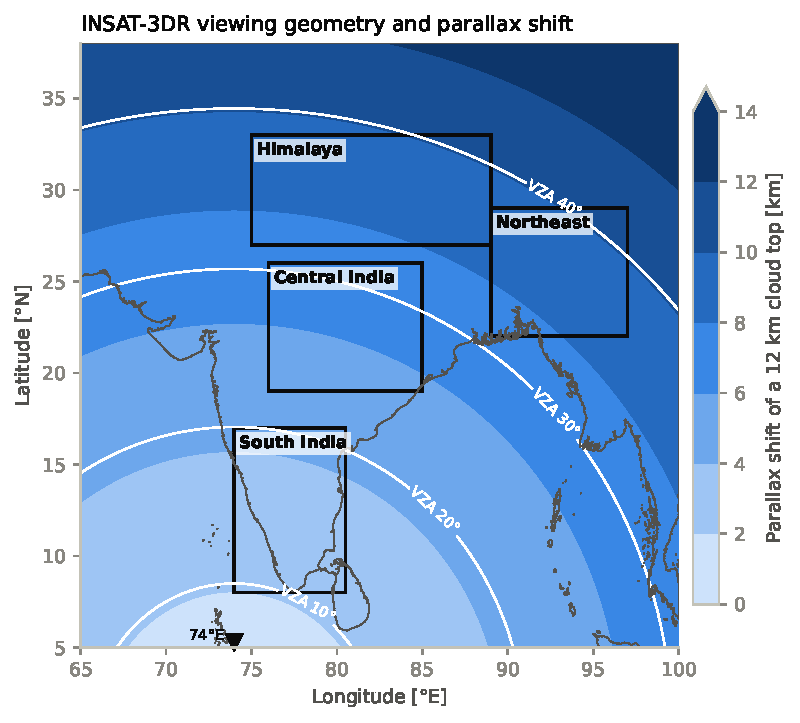
\includegraphics[width=0.8\textwidth]{figures/fig1_geometry.pdf}
  \caption{INSAT-3DR viewing geometry over South Asia. Colours: parallax shift of a 12\,km cloud top, $h\tan(\mathrm{VZA})$; white lines: viewing zenith angle. Boxes: the four validation regions. The sub-satellite point is at 74\,\textdegree E.}
  \label{fig:1}
\end{figure}

\begin{figure}[tbp]
  \centering
  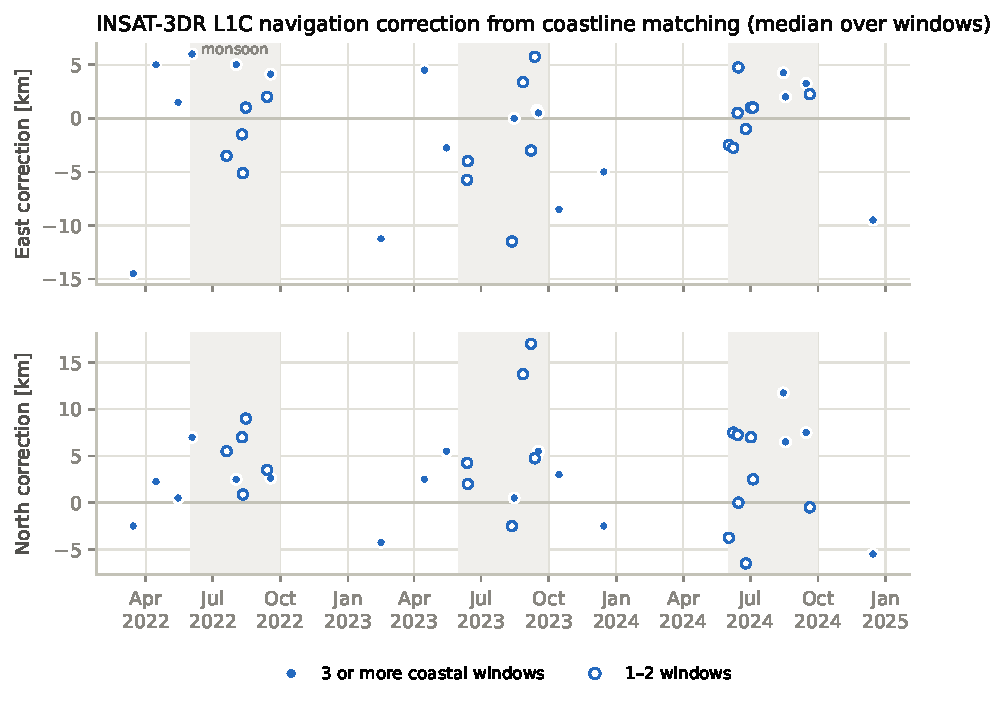
\includegraphics[width=\textwidth]{figures/fig2_navigation.pdf}
  \caption{INSAT-3DR L1C navigation correction from coastline matching, March 2022 to December 2024 (median over the accepted coastal windows of each date). Filled points: three or more windows; open points: one or two. Shading: June--September. Positive values mean INSAT positions must move east or north.}
  \label{fig:2}
\end{figure}

\begin{figure}[tbp]
  \centering
  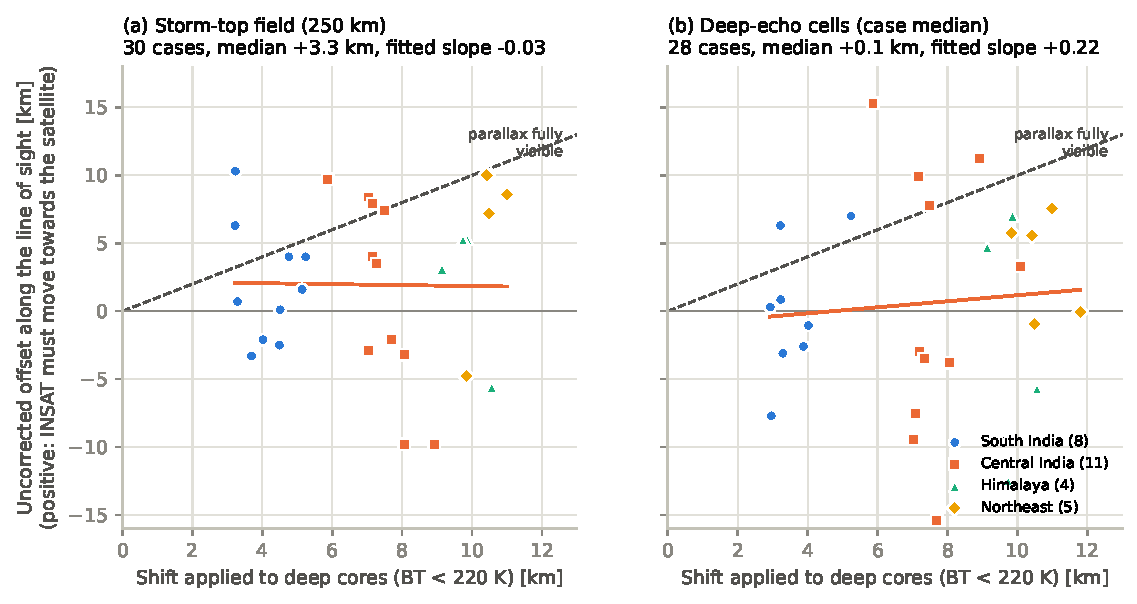
\includegraphics[width=0.9\textwidth]{figures/fig3_cases.pdf}
  \caption{Line-of-sight offset between INSAT and GPM (storm-top field, 250\,km window) for each case before (open) and after (filled) parallax correction, ordered by viewing zenith angle (in brackets). Positive: INSAT must move towards the satellite to match GPM.}
  \label{fig:3}
\end{figure}

\begin{figure}[tbp]
  \centering
  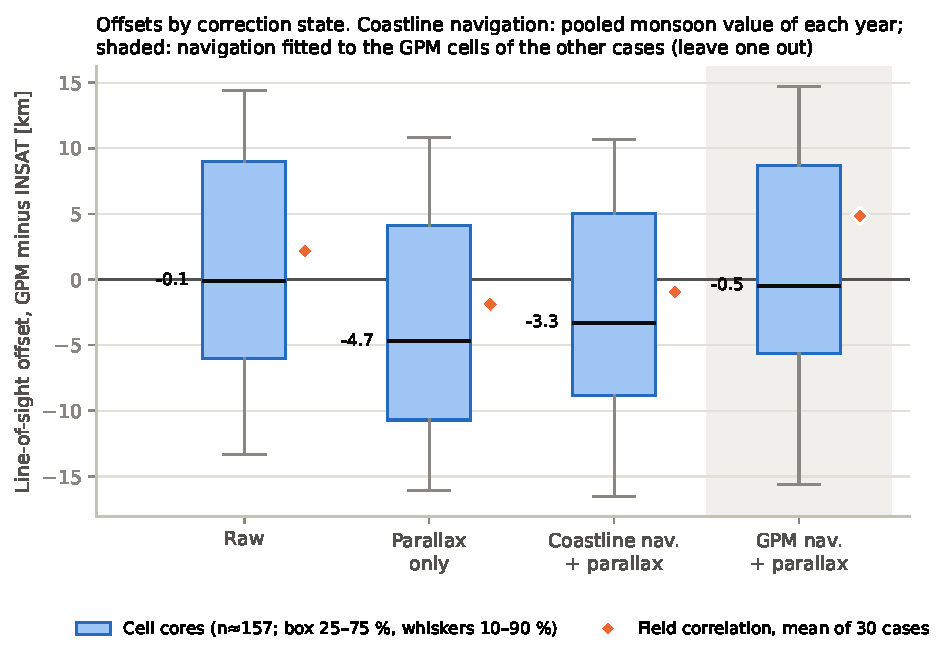
\includegraphics[width=\textwidth]{figures/fig4_states.pdf}
  \caption{Line-of-sight offsets in each correction state. Boxes: cell-by-cell offsets between GPM deep-echo cells and INSAT cold cores (box 25--75\,\%, whiskers 10--90\,\%; median labelled). Diamonds: mean field-correlation offset over 12 cases. Navigation: near-storm monsoon correction ($-0.5$\,km E, $+2.5$\,km N); shaded: all-India monsoon median ($+1.8$\,km E, $+4.8$\,km N) as a sensitivity test.}
  \label{fig:4}
\end{figure}

\begin{figure}[tbp]
  \centering
  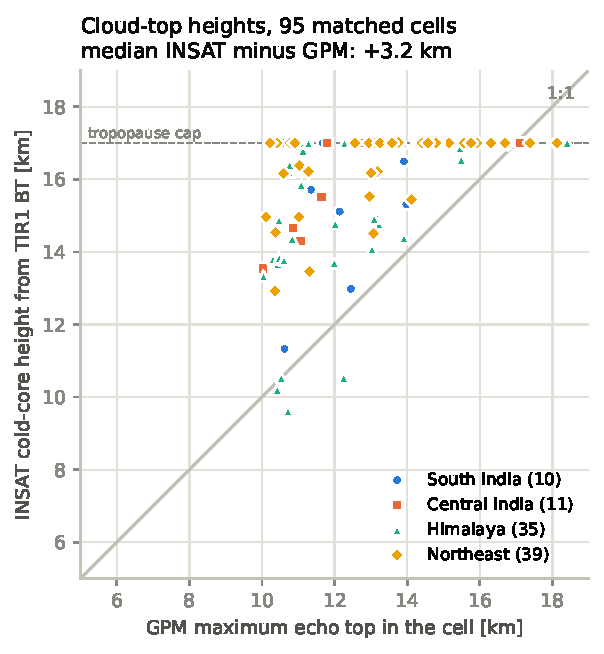
\includegraphics[width=0.6\textwidth]{figures/fig5_heights.pdf}
  \caption{Cloud-top height of the INSAT cold core (from TIR1 brightness temperature, AFGL tropical profile) against the GPM maximum echo top in the same cell, for 95 matched cells. Dashed line: the tropopause cap of the profile.}
  \label{fig:5}
\end{figure}

\begin{figure}[tbp]
  \centering
  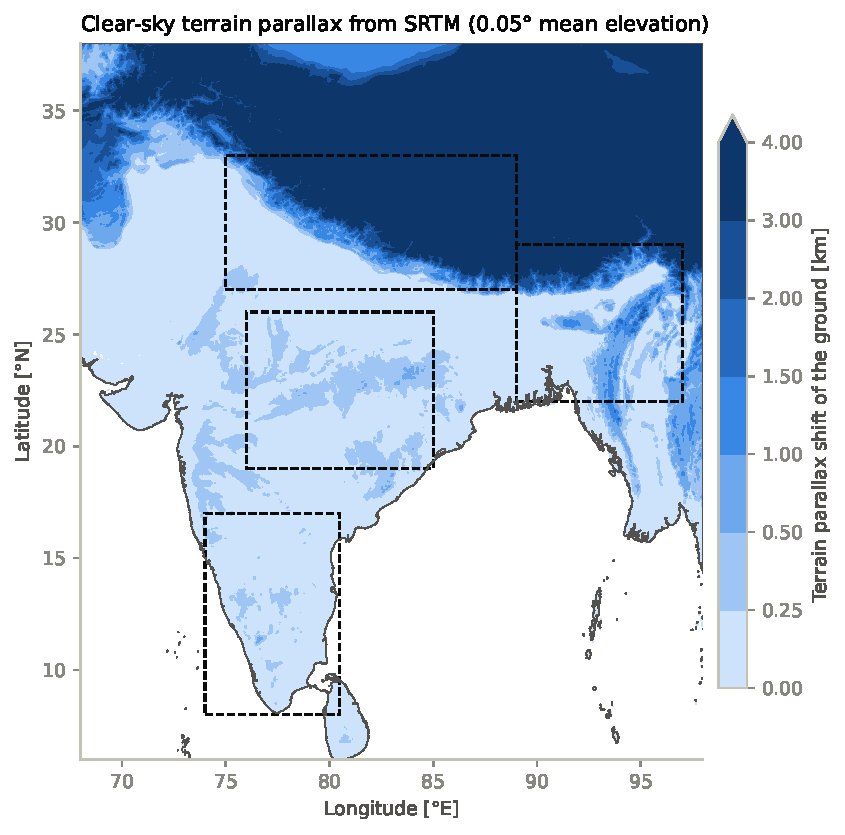
\includegraphics[width=0.8\textwidth]{figures/fig6_terrain.pdf}
  \caption{Clear-sky terrain parallax: displacement of the ground in ellipsoid-navigated INSAT-3DR imagery, from SRTM elevation averaged to 0.05\,\textdegree. Dashed boxes: validation regions.}
  \label{fig:6}
\end{figure}

\section{Discussion}
\label{sec:discussion}
\label{sec:6}

\subsection{What the correction achieves}\label{sec:6.1}

The ellipsoid ray-tracing correction is exact to well under the pixel size, and its effect on real data is the one geometry predicts: features move along the line of sight by h·tan(VZA), and nothing moves across it. Against GPM, the correction halves the typical INSAT--radar offset (5.5 → 3.1 km), and together with the monsoon navigation correction brings it to 1.8 km. The gain is largest where it matters most, over the Himalaya and Northeast India, where the parallax of deep convection (about 10 km) is two to three INSAT pixels.

\subsection{Navigation partly masks the parallax}\label{sec:6.2}

The most important finding for users of INSAT-3DR data is that the raw INSAT--GPM offset does not follow the viewing angle. In the monsoon, a navigation error of 2.5--5 km to the south partly offsets the northward parallax displacement, so uncorrected cold cores sit close to the radar cells (Section~\ref{sec:5.5}). A correction that removes only the parallax therefore overshoots at storm cores.

Two practical consequences follow:

\begin{itemize}
\tightlist
\item
  Parallax and navigation should be corrected together. The navigation error is seasonal: small in the monsoon, but 7--20 km to the west from late September to mid-March, larger than the parallax itself. Users of INSAT-3DR outside the monsoon need the seasonal correction even more than the parallax correction.
\item
  The monsoon navigation error cannot be measured for a single day from coastlines, because clouds hide the coasts and night-time land--sea contrast is too weak. A seasonal value, with its ±2 km uncertainty, is the best available. Other landmarks (lakes, rivers, islands) or ISRO's own navigation reports could reduce this uncertainty.
\end{itemize}

\subsection{Which cloud height to use}\label{sec:6.3}

Brightness-temperature heights put the coldest convective tops at the tropopause, about 4.4 km above the GPM echo tops, with either the standard atmosphere or ERA5. This is mainly physical: the infrared signal comes from the top of the cloud, while the radar sees large precipitation particles lower down. The consequence depends on the application:

\begin{itemize}
\tightlist
\item
  For \textbf{cloud products} (cloud masks, cloud-top properties), the infrared top is the right height, and the correction places the cloud where it is.
\item
  For \textbf{precipitation products}, the rain-relevant level lies below the infrared top. Correcting with the full cloud-top height moves the cold signal slightly past the rain core, which may explain part of the remaining cell-measure offset. An effective height below the infrared top could fit precipitation better; we leave this to future work.
\end{itemize}

ISRO's operational cloud-top pressure product, by contrast, placed deep cores 2--3 km lower than the BT heights in our first case (Kochi, 6 June 2022; r = 0.86 overall) and was not used for the correction.

\subsection{Terrain}\label{sec:6.4}

Terrain does not affect the storm results but matters for anything observed at the ground in clear sky. Over the Himalaya, ellipsoid-navigated pixels of high terrain are misplaced by several kilometres; for land-surface temperature, snow cover or surface classification in mountains, terrain-aware correction should be standard.

\subsection{Relation to earlier work}\label{sec:6.5}

\citet{vicente2002} showed that parallax and orographic corrections matter for satellite rainfall estimates from GOES; our results confirm the size of the effect for INSAT-3DR over India, where the high viewing angles over the Himalaya and the Northeast make it about 10 km for deep convection. The solver follows \citet{bielinski2020}, extended here to terrain and to a navigation correction measured from coastlines. The GOES Hydro-Estimator has applied the \citet{vicente2002} correction operationally since 2001, and satpy \citep{satpy_parallax} offers an open-source spherical-Earth correction for gridded geostationary data. To our knowledge, however, no parallax correction or validation has been published for INSAT-3D or INSAT-3DR.

ISRO's data-quality reports \citep{mosdac_dqe2020} already measure INSAT-3DR geolocation error per image against ground control points; for a full-disk L1B image of 19 June 2020 they give a mean error of about 2.6 IR pixels to the north and 1.0 pixel to the west. Our coastline estimate for the 2022--2024 monsoon L1C data is smaller (2.5--5 km to the north) but has the same direction; the products, years and methods differ. What is new here is the multi-year seasonal behaviour of the L1C error and its interaction with the parallax: in the monsoon the two partly cancel, so a parallax-only correction overshoots, and the navigation error cannot be measured for a single day. \emph{(See \texttt{00\_Documentation/novelty\_check.md}; confirm with a Google Scholar / Scopus search before submission.)}

\subsection{Limitations}\label{sec:6.6}

\begin{itemize}
\tightlist
\item
  \textbf{Sample size.} Fourteen usable cases (12 for the field measure) are enough to show the effect but not to give tight regional statistics. South and Central India have only 1--3 cases each.
\item
  \textbf{One reference instrument.} Validation uses GPM only. GPM samples each storm once, in a 245 km swath, and its echo tops differ from infrared tops by definition. Ground-based radar (IMD Doppler Weather Radar) would add many more cases at fixed sites and is left for future work.
\item
  \textbf{Two measures, one gap.} The field and cell measures differ by a steady 4--5 km because they compare different parts of the storm. We report both; the absolute residual offset is therefore uncertain by about ±2--3 km.
\item
  \textbf{Navigation.} The monsoon navigation correction is a seasonal value with an uncertainty of about ±2 km; the yaw-flip explanation of its seasonal change is a hypothesis.
\item
  \textbf{Cloud height.} Heights come from TIR1 brightness temperature, which underestimates thin cirrus and cannot resolve overshooting tops above the tropopause.
\end{itemize}

\subsection{Effect on precipitation-type classification}\label{sec:6.7}

\emph{To be written after the U-Net comparison (Model A uncorrected vs Model B corrected, on the designed test set of 91 scenes).}


\section{Conclusions}
\label{sec:conclusions}

We have presented PyGeoParallax-IN, an open-source tool that corrects INSAT-3DR imagery for cloud parallax by exact ray tracing on the WGS84 ellipsoid, with optional terrain and a navigation correction measured from coastlines, and validated it against GPM radar over monsoon India.

\begin{enumerate}
  \item \textbf{The correction is exact and behaves as geometry predicts.} It agrees with independent implementations to within millimetres to tens of metres, moves features only along the line of sight, and moves deep convection by 4\,km over South India and about 10\,km over the Himalaya and Northeast India.
  \item \textbf{It improves agreement with GPM.} The median storm-top offset falls from 5.5 to 3.1\,km with parallax correction (10 of 12 cases improve; sign test $p=0.039$, moderate evidence), and the cross-look offset does not change. With the navigation correction as well the median is 1.8\,km, but 12 cases cannot show that this further step is significant.
  \item \textbf{INSAT-3DR navigation must be corrected together with parallax.} The L1C navigation error is seasonal: 7--20\,km to the west from late September to mid-March, and 2.5--5\,km to the south in the monsoon. In the monsoon it partly cancels the parallax, so a parallax-only correction overshoots significantly at storm cores ($-5.7$\,km, 95\,\% interval $-8.2$ to $-2.2$\,km); adding the navigation correction reduces the overshoot significantly. The error cannot be measured for a single day from coastlines, and a seasonal correction with an uncertainty of about $\pm2$\,km is the best available.
  \item \textbf{Cloud height and terrain are secondary for storms.} Brightness-temperature heights of the coldest tops lie at the tropopause with either the standard atmosphere or ERA5, about 4.4\,km above the GPM echo tops; this is a physical difference between infrared and radar tops. Terrain changes the storm results by less than 0.1\,km but moves clear-sky ground in the Himalaya by up to 6\,km.
  \item \textbf{The tool is fast and ready for downstream use.} It processes an India scene in 1.8\,s and writes uncorrected and corrected datasets that are identical in clear sky.
\end{enumerate}

Users of INSAT-3DR imagery over India, especially at high viewing angles, should correct navigation and parallax together. Future work will add validation cases, especially over South and Central India, to settle the effect of the navigation correction and the dependence on viewing angle; extend the validation to ground-based radar (IMD Doppler Weather Radar), test an effective height for precipitation products, and quantify the effect of the correction on precipitation-type classification. The code, scripts and validation case lists are available at \url{https://github.com/bapallinaveen60/PyGeoParallax-IN}.


\section*{Code availability}
{\sloppy
PyGeoParallax-IN (version 0.4.0, MIT licence), with the scripts, case lists and U-Net training and comparison scripts used in this study, is archived on Zenodo \citep{pygeoparallax}: \doi{10.5281/zenodo.23812270}. The concept DOI, \doi{10.5281/zenodo.23666957}, always resolves to the latest version. Development continues at \url{https://github.com/bapallinaveen60/PyGeoParallax-IN}.\par}

\section*{Data availability}
{\sloppy
INSAT-3DR Imager L1C and L2B products are available from MOSDAC, Space Applications Centre, ISRO (\url{https://www.mosdac.gov.in}) after free registration. GPM DPR 2A Ku version 8 data are available from NASA GES DISC \citep{gpm2aku_v08}. ERA5 pressure-level data are available from the Copernicus Climate Data Store \citep{c3s2018}. SRTM elevation data \citep{farr2007} were obtained through OpenTopography, and coastlines from Natural Earth \citep{naturalearth}. The validation case list (GPM orbits and INSAT scan times) is part of the code archive above.\par}

\section*{Author contributions}
NB designed the study, wrote the software, carried out the validation and the U-Net experiments, and wrote the manuscript.

\section*{Competing interests}
The author has declared that there are no competing interests.

\section*{Acknowledgements}
{\sloppy
INSAT-3D and INSAT-3DR data were provided by the Meteorological and Oceanographic Satellite Data Archival Centre (MOSDAC), Space Applications Centre, ISRO. GPM data were provided by the NASA/JAXA Global Precipitation Measurement mission through the NASA Goddard Earth Sciences Data and Information Services Center (GES DISC). ERA5 was produced by the European Centre for Medium-Range Weather Forecasts (ECMWF) and made available by the Copernicus Climate Change Service. SRTM data were provided by NASA and USGS through OpenTopography, and coastlines by Natural Earth. The software builds on NumPy, SciPy, xarray, pyproj, Numba, h5py and TensorFlow; satpy and pyorbital were used for independent checks. The author thanks the developers of the attention U-Net and of the labelled INSAT--GPM patches used in Section~\ref{sec:4.8}. An AI assistant (Claude, Anthropic) was used to help write code and edit the text; the author reviewed all of it and takes full responsibility for the content.\par}

\section*{Financial support}
This research received no external funding.

\bibliographystyle{plainnat}
\bibliography{references}

\end{document}
